
\section{Background}
\label{sec:background}

With increasing traffic on telecommunications networks, effectively balancing the load across all nodes of the network is crucial to the network performing well. In other words, while shortest path algorithms may quickly find the optimal short-distance route between nodes in a call, an improved algorithm will bypass high congestion areas in order to make calls more efficient and avoid dropping calls on the network. In order to effectively balance loads, we look to the previous research done by Ruud Schoonderwoerd, Owen Holland, Janet Bruten, and Leon Rothkrantz on simulating pheromone trails of ants. As real-life ants follow paths, they drop pheromones to influence the behavior of other ants and improve the overall colony’s sense of navigation. The strength of the pheromones decreases over time, so ants that find paths that take less time have a larger influence on the paths taken by future ants. \\

\begin{figure}[htb]

  \centering
  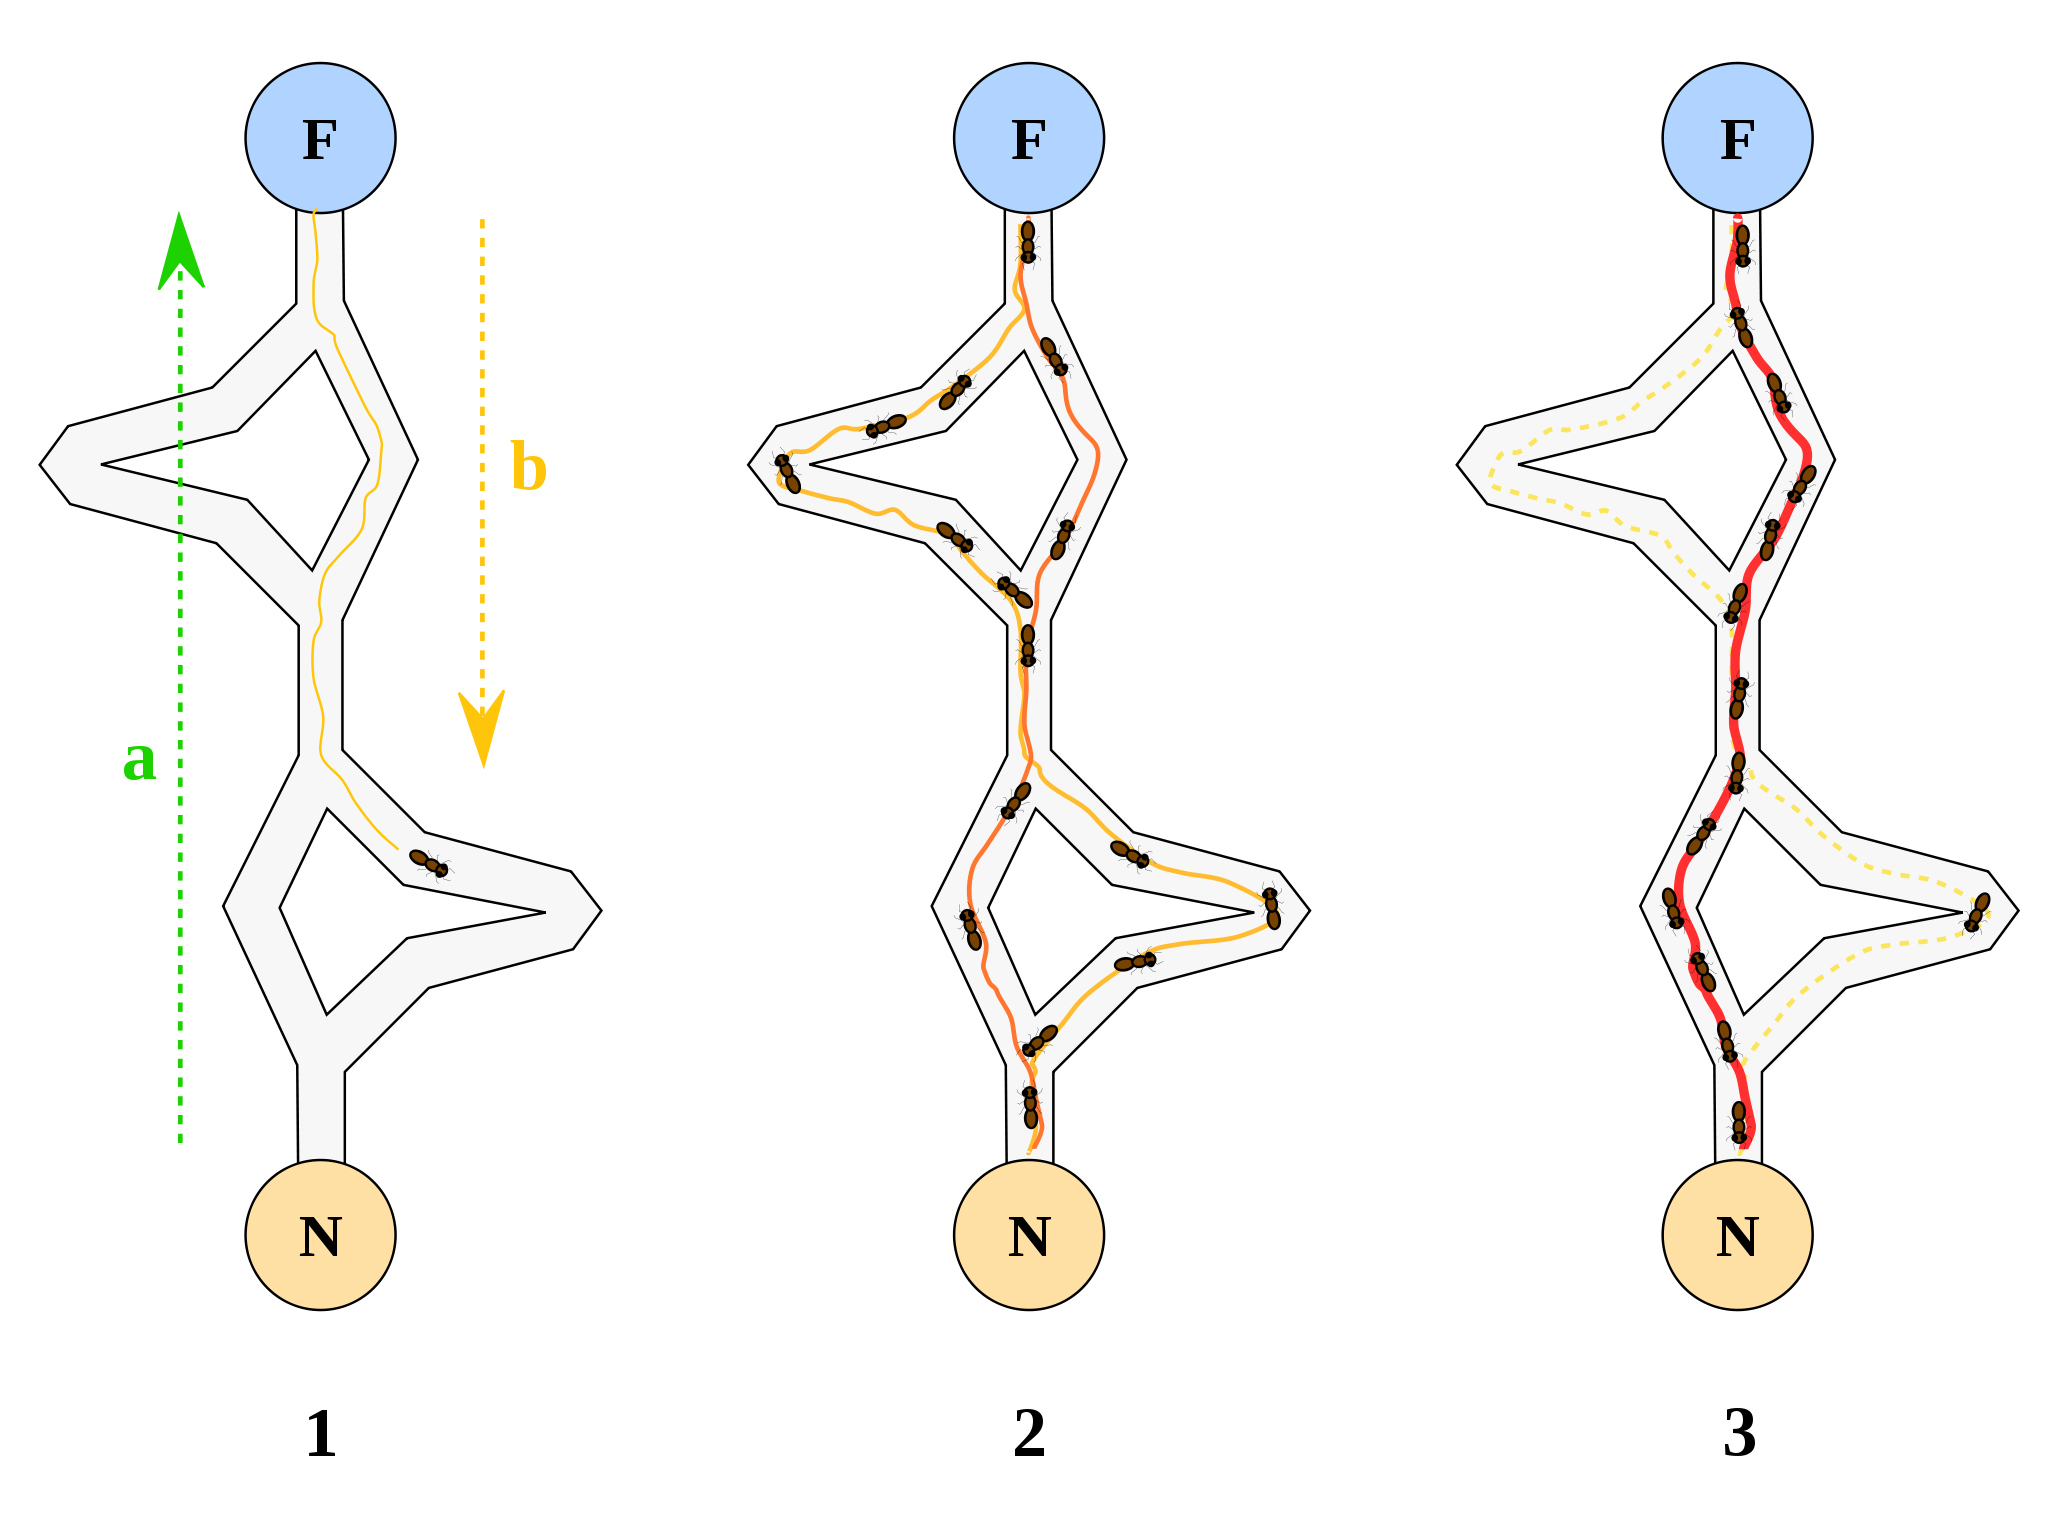
\includegraphics[width=0.47\textwidth]{figs/ants_nature.jpg}
  \caption{An example of ant colony routing over time. (Wikimedia Commons)}
  \label{fig:tex}

\end{figure}

Our algorithm adopts this approach using artificial ant-like agents to regulate local call routing. Ants become delayed on congested nodes, and have decaying influence on routing probabilities as a function of time spent on the network. The theory is that as an ant travels along a path, if the path is congested, the ant's pheromones will be weaker, so ants (and network calls) traveling in the future will be less likely to take that path.